\documentclass[conference]{IEEEtran}
\usepackage{graphicx}
\usepackage{hyperref}
\usepackage{url}
\usepackage{amsmath}
\usepackage{booktabs}
\usepackage{listings}
\usepackage{xcolor}
\usepackage{subcaption}

\hypersetup{
  colorlinks=true,
  linkcolor=blue,
  urlcolor=blue,
  citecolor=blue,
}

\Urlmuskip=0mu plus 2mu
\emergencystretch=1.5em
\newcommand{\code}[1]{\nolinkurl{#1}}
\newcommand{\runlabel}[1]{\medskip\noindent\textit{#1}\par}

\lstset{
  basicstyle=\ttfamily\scriptsize,
  breaklines=true,
  breakatwhitespace=false,
  breakindent=0pt,
  columns=fullflexible,
  keepspaces=true,
  frame=tb,
  framerule=0.4pt,
  framesep=3pt,
  xleftmargin=4pt,
  xrightmargin=4pt,
  framexleftmargin=0pt,
  framexrightmargin=0pt,
  backgroundcolor=\color{gray!10},
  postbreak=\mbox{\textcolor{red}{$\hookrightarrow$}\space},
  aboveskip=4pt,
  belowskip=4pt,
}

\title{Offloading the 5G UPF User-Plane Datapath to NVIDIA BlueField-3 with DOCA Flow}

\author{%
  \IEEEauthorblockN{Plabon Dutta}
  \IEEEauthorblockA{Department of Computer Science\\
  University of Kentucky\\
  plabon.dutta@uky.edu}
}

\begin{document}
\maketitle
\thispagestyle{plain}
\pagestyle{plain}


% ─────────────────────────────────────────────────────────────────────
\begin{abstract}
We describe a hardware-offload subsystem for the user-plane datapath
of L25GC-plus, an open-source 3GPP-compliant 5G core.  Using the
NVIDIA DOCA Flow SDK, we push per-UE classification and GTP-U
decap/encap entirely into the BlueField-3 DPU's integrated
ConnectX-7 steering engine, taking the host CPU out of the fast
path.  A \emph{split-agent} design relays PFCP-derived rule messages
from a host-side ONVM NF (host\_agent) to a native DPU-side
application (dpu\_agent) over DOCA Comch; the DPU side builds and
maintains the hardware pipeline on the BF3 ARM cores.  With this
design --- hardware classification plus hardware GTP-U decap/encap,
and no software fallback datapath --- the offloaded UPF reaches line
rate on a 100~GbE PF in both directions simultaneously under
two-sided DPDK Pktgen at 1024-byte frames, with zero reported packet
errors.  Control-plane benchmarks up to 2{,}000{,}000 rules measure
9{,}100--9{,}200 rule inserts/s and 780{,}000--975{,}000 rule
deletes/s, with insert rate steady as the table grows.  DL packet
buffering and GBR traffic shaping are implemented but not yet
validated on hardware; their designs are described here for later
validation.
\end{abstract}

% ─────────────────────────────────────────────────────────────────────
\section{Introduction and Motivation}

A software-based 5G UPF running on commodity x86 CPUs scales poorly at
multi-gigabit line rates.  Per-packet costs (PCIe DMA, cache misses,
and software scheduling) grow linearly with traffic and are hard to
amortize at 100~Gbps.

The NVIDIA BlueField-3 (BF3) is a SmartNIC with integrated
ConnectX-7 networking (the model used here exposes two 100~GbE
physical-function ports) whose embedded ARM cores can run
programmable packet-processing logic alongside the host CPU.  Its
eSwitch supports hardware flow steering through the DOCA Flow API,
so GTP-U tunnel termination, metering, and encapsulation can run
entirely in the NIC ASIC and the host CPU sees no fast-path packets.

\paragraph{Where the software UPF actually spends its time.}
Before deciding which stages of the UPF datapath are worth
offloading, we profiled the per-packet cost of the existing
single-core software UPF (ONVM-UPF, the user-plane component of
L25GC-plus).  Table~\ref{tab:swupf-profile} breaks the fastpath into
its constituent steps and reports the average time per step and its
share of the total per-packet cost.

\begin{table}[!h]
  \centering
  \caption{Per-packet cost breakdown of the software UPF fastpath
           (single x86 core).}
  \label{tab:swupf-profile}
  \footnotesize
  \setlength{\tabcolsep}{4pt}
  \begin{tabular}{@{}lrrr@{}}
    \toprule
    Step                                 & Time (ns) & Cycles  & \% of total \\
    \midrule
    IPv4 header parse                    &  19.8     &   51.4  &  2.34 \\
    Direction discrimination             &  40.8     &  105.9  &  4.81 \\
    GTP-U parse (UL)                     &  19.5     &   50.6  &  2.30 \\
    Match-key build                      &  35.5     &   92.1  &  4.19 \\
    \textbf{PDR classification}          & \textbf{514.9} & \textbf{1335.4} & \textbf{60.76} \\
    QER flow lookup                      &  10.3     &   26.8  &  1.22 \\
    UE QoS lookup                        &  12.4     &   32.1  &  1.46 \\
    Strip outer L2                       &  13.0     &   33.6  &  1.53 \\
    GTP-U decap (UL)                     &   8.3     &   21.6  &  0.98 \\
    \textbf{FAR + GTP-U encap (DL)}      & \textbf{83.8}  & \textbf{217.3}  &  \textbf{9.88} \\
    Attach outer L2                      &  20.7     &   53.8  &  2.44 \\
    QoS metering (trTCM)                 &  20.4     &   52.9  &  2.41 \\
    \midrule
    \textbf{Total}                       & \textbf{847.6} & \textbf{2198.4} & \textbf{100} \\
    \bottomrule
  \end{tabular}
\end{table}

Two stages dominate.  \emph{PDR classification} --- the per-packet
match-table lookup that selects the right rule for an arriving
packet --- alone accounts for $\sim$61\% of the per-packet cost.
\emph{DL FAR + GTP-U encapsulation} adds another $\sim$10\%.
Together these two stages account for roughly 70\% of the software
fastpath.  Both map cleanly onto NIC steering primitives:
classification becomes a DOCA Flow match pipe (with the per-rule
meter attached as a side action), and DL encap becomes a hardware
GTP-U + PSC encap action on the egress port.  Pushing them into the
BF3 ASIC removes them from the host's per-packet budget entirely,
which is the primary quantitative justification for the offload
described in the rest of this report.

The goal of this work is to build a hardware-accelerated forwarding
plane for ONVM-UPF~\cite{onvm} that:
\begin{enumerate}
  \item Offloads UL GTP-U decapsulation and DL GTP-U encapsulation to BF3
        hardware.
  \item Supports per-UE QoS enforcement (trTCM metering, GBR shaping).
  \item Supports PDR buffering for UE idle-mode transitions
        (\texttt{BUFF}/\texttt{FORW} FAR actions).
  \item Stays out of the way of un-offloaded traffic: any packet that
        misses the offloaded rules takes the DOCA Flow default VNF
        miss path (RSS on its ingress PF) and is delivered to the
        host stack.
\end{enumerate}

% ─────────────────────────────────────────────────────────────────────
\section{Background: DOCA Flow}
\label{sec:bg}

This section covers the parts of the NVIDIA DOCA Flow
SDK~\cite{doca} needed to follow the rest of the report.  See the
official DOCA documentation~\cite{doca} for a full reference.

\subsection{What DOCA Flow Is}

DOCA Flow is the lowest-level NVIDIA API for building generic
hardware-accelerated packet-processing pipelines on ConnectX/BlueField
NICs.  An application using DOCA Flow describes packet processing as
a graph of \emph{pipes}, each pipe consisting of:

\begin{itemize}
  \item \textbf{Match}: which packet fields a pipe inspects (Ethernet,
        VLAN, IPv4/IPv6, TCP/UDP/ICMP, GRE/VXLAN/GTP-U/ESP/PSP, and
        per-packet metadata).
  \item \textbf{Monitor}: counters and trTCM meters/policers attached
        to entries.
  \item \textbf{Modify (Actions)}: header rewrites such as MAC/IP/L4
        modification, tunnel add/strip, set-metadata,
        encrypt/decrypt.
  \item \textbf{Forward (FWD)}: where matched packets go next ---
        another pipe, a port (wire / representor), an RSS queue set
        (software path), or DROP.
\end{itemize}

Pipes are templates (created once); per-rule \emph{entries} are then
inserted into a pipe and represent a specific HW flow rule with
concrete match values and forward target.  Packets that miss every
entry of a pipe are routed by the pipe's \texttt{fwd\_miss} rule (or
by the per-domain default miss behavior).

\subsection{Pipe Modes: VNF vs. Switch}

DOCA Flow supports two main \emph{pipe modes}, set via the
\code{mode_args} string at port initialization.  The mode determines
the topology of the underlying steering graph and the default miss
behavior:

\begin{itemize}
  \item \textbf{VNF mode}: targets virtual-network-function use cases.
        Each physical/virtual port is a first-class DOCA Flow port,
        and packets that miss are sent to the host's RSS queues by
        default.  Forwarding between ports is explicit: the
        application calls \code{doca_flow_port_pair(X, Y)} to
        unidirectionally pair port~X to port~Y.  Cross-domain
        forwarding from an ingress pipe to an egress pipe is
        permitted only if the egress pipe is the EGRESS-domain
        \emph{root}.  Software-Tx packets traverse only the EGRESS
        pipeline of the Tx port; they do \emph{not} re-enter the
        ingress ROOT pipe.

  \item \textbf{Switch mode}: targets internal switching between
        representor ports (uplink representors, SF/VF representors).
        DOCA Flow unifies all ports under a single ``switch manager''
        port that owns the pipeline, and missed traffic is delivered
        to RSS on that manager.  VF/SF representor ports must
        \emph{not} be initialized through the DPDK API in this mode.
\end{itemize}

This project uses VNF mode (\code{mode_args = "vnf,hws"}).  An earlier
iteration of the codebase ran in switch mode, and the move to VNF
came out of a concrete set of problems rather than an abstract
preference.

Switch mode is representor- and eSwitch-manager-centric: pipeline
ownership lives on the switch manager port, and cross-port forwarding
flows through representor handles rather than directly between the
ingress PFs.  Our deployment has neither uplink representors nor
SF/VF representors in the data plane --- just two physical-function
ports, N3 (PF0) and N6 (PF1) --- so we were forcing a clean PF-to-PF
VNF topology onto a representor-centric model.  The mismatch
produced two recurring problems.  First, UL-decapped traffic on N3
did not always steer reliably to N6, because the natural egress
port was reached indirectly via the switch manager rather than
directly from the ingress PF that decapped the packet.  Second, the
interaction of the root pipe, the FDB context, and the EGRESS domain
was hard to reason about, which made slow-path reinject assumptions
particularly fragile.

VNF mode matches the deployment.  Each PF becomes a first-class DOCA
Flow port, paired explicitly with \code{doca_flow_port_pair(N3, N6)}
and \code{doca_flow_port_pair(N6, N3)}.  UL pipes live naturally on
the N3 ingress side, DL pipes live naturally on the N6 ingress side,
and cross-port forwarding is explicit instead of implicit through a
switch manager.

VNF mode also exposed the constraint that drove most of the
slow-path redesign.  Software Tx on a port traverses only that port's
EGRESS pipeline; it does \emph{not} re-enter the ingress ROOT.  The
buffer and shaper paths in earlier revisions relied on reinjection
and that approach simply did not work in VNF mode.  The current
design (Sections~\ref{sec:buffering} and~\ref{sec:shaping}) reflects
this: DL\_ENCAP lives on the N3 EGRESS root; the buffer lcore
finalizes the wire-form packet in software and transmits on N3; UL
YELLOW shaping decaps in software and transmits on N6; DL YELLOW
shaping encaps in software and transmits on N3.  Switch mode was
fighting the topology; VNF mode matched it but in turn forced this
software-finalization design for slow-path traffic.

\subsection{Hardware Steering vs.\ Software Steering}

DOCA Flow can run in either \emph{Hardware-Steering} (HWS) or
\emph{Software-Steering} (SWS) mode, also selected via
\code{mode_args}.  HWS pushes match/action evaluation into the NIC's
flow-steering engine, removing the per-packet ARM-core involvement
that SWS requires.  This project uses HWS exclusively
(\code{mode_args = "vnf,hws"}); SWS is mentioned only for completeness.

\subsection{Steering Domains}

DOCA Flow groups pipes into four steering \emph{domains} that
constrain which actions are legal and how miss behavior is defined:

\begin{itemize}
  \item \texttt{DOCA\_FLOW\_PIPE\_DOMAIN\_DEFAULT}: ingress traffic;
        non-secure actions only; default miss is DROP.  The next
        legal milestone is a queue (RSS) or a pipe in the EGRESS
        domain.
  \item \texttt{DOCA\_FLOW\_PIPE\_DOMAIN\_SECURE\_INGRESS}: only
        domain that may host decrypt actions; encap/encrypt are
        forbidden.
  \item \texttt{DOCA\_FLOW\_PIPE\_DOMAIN\_EGRESS}: egress traffic;
        non-secure actions only; default miss is ``send to wire /
        representor''.
  \item \texttt{DOCA\_FLOW\_PIPE\_DOMAIN\_SECURE\_EGRESS}: only
        domain that may host encrypt actions; decap is forbidden.
\end{itemize}

Domain transitions are not arbitrary: traffic moves DEFAULT $\to$
EGRESS only via a forward into the EGRESS-root pipe, and the reverse
direction is not allowed.  This is why, in our pipeline, the
DL\_ENCAP pipe is built on the N3 EGRESS-root: it is the only place
where GTP-U encapsulation can occur on the egress wire, and DL pipes
in the DEFAULT domain on N6 forward into it via cross-domain
\code{FWD_PIPE}.

\subsection{Per-Packet Metadata (\texttt{pkt\_meta})}

DOCA Flow exposes a per-packet 32-bit metadata field that pipes can
read and write as part of match and action.  In our design,
UL\_MATCH and DL\_MATCH stamp \code{pkt_meta=htonl(hw_rule_id)} on
matched packets; downstream pipes (color gate, DL\_ENCAP) then
match on \code{pkt_meta} to identify the originating rule without
re-parsing headers.  This is the cross-pipe correlation key used
throughout the pipeline.

% ─────────────────────────────────────────────────────────────────────
\section{Testbed and Experimental Setup}
\label{sec:testbed}

\subsection{FABRIC Testbed}

All experiments are conducted on the FABRIC~\cite{fabric} research testbed.
A three-node slice is provisioned using the custom Jupyter notebook
\code{L25GC_DPU_BF3_3node_complete.ipynb}.

\begin{itemize}
  \item \textbf{UERAN node}: Runs UERANSIM to emulate a 5G base station (gNB)
        and UEs.
  \item \textbf{CN node}: Runs the L25GC-plus 5G core network
        (AMF, SMF, etc.)~\cite{l25gcplus,l25gc,l25gc_rethink} together
        with ONVM-UPF on the x86 host.  L25GC-plus is an open-source,
        3GPP-compliant 5G core developed for low-latency control-plane
        operations; the BF3 hardware-offload work in this report
        targets its user-plane datapath.  The BF3 DPU is physically
        attached to this node.
  \item \textbf{DN node}: Acts as the data-network (internet) endpoint.
\end{itemize}

\subsection{Hardware and Software}

\begin{itemize}
  \item \textbf{DPU}: NVIDIA BlueField-3 with integrated
        ConnectX-7 networking (Mellanox \texttt{MT43244},
        \texttt{mlx5\_core} driver), configured as two 100~GbE
        physical functions: PF0 at \texttt{03:00.0} (N3) and PF1 at
        \texttt{03:00.1} (N6).  Each PF is a 100~GbE wire; the
        throughput numbers in Section~\ref{sec:throughput} are
        per-direction over one such port.
  \item \textbf{DOCA SDK}: Version 3.3 (\texttt{vnf,hws} pipeline mode).
  \item \textbf{UPF}: ONVM-UPF, a DPDK secondary process (NF) running on
        the x86 host under OpenNetVM~\cite{onvm}.
  \item \textbf{Build system}: Meson/Ninja (dpu\_agent is built natively on
        the BF3 ARM; host-side components are cross-compiled on x86).
\end{itemize}

\subsection{Network Topology}

\begin{itemize}
  \item \textbf{N3 interface}: Between UERAN node and the BF3 PF0
        (\texttt{03:00.0}, DOCA Flow port~0).  Carries GTP-U tunnels.
  \item \textbf{N6 interface}: Between the BF3 PF1 (\texttt{03:00.1},
        DOCA Flow port~1) and the DN node.  Carries inner UE IP traffic.
\end{itemize}

The x86 host kernel owns the UPF IP addresses; BF3 runs in promiscuous mode
so it can intercept all N3/N6 traffic for hardware processing.

% ─────────────────────────────────────────────────────────────────────
\section{Split-Agent Architecture}

The offload subsystem follows a \emph{split-agent} design (see
Fig.~\ref{fig:arch}).  Control intelligence (PFCP session handling)
stays on the x86 UPF-C, and data-plane rule programming is delegated
to the BF3 ARM via a lightweight message protocol.

This split also enables \emph{proactive} rule installation.  PFCP
signalling on the x86 side (Create / Update / Remove PDR / FAR / QER
from the SMF) drives HW rule installs at session-establishment time,
before any user-plane traffic for the UE has arrived.  By contrast,
the NVIDIA DOCA Sample UPF Accel application is reactive: the first
packet of every new flow misses in hardware, takes a software path
that installs the matching rule on demand, and only subsequent
packets of that flow are HW-accelerated.  Programming rules
proactively means the very first user-plane packet of a flow already
matches a HW entry; there is no per-flow first-packet penalty and no
need for a permanent software fallback datapath alongside the
offload.  This is why the pipeline (Section~\ref{sec:pipeline}) does
not include a dedicated software-fallback pipe: the only way a packet
goes to the host is via the DOCA Flow default VNF miss path, which
should normally be exercised only by control traffic and by packets
that arrive before their session's rules have been installed.

\begin{figure*}[t]
  \centering
  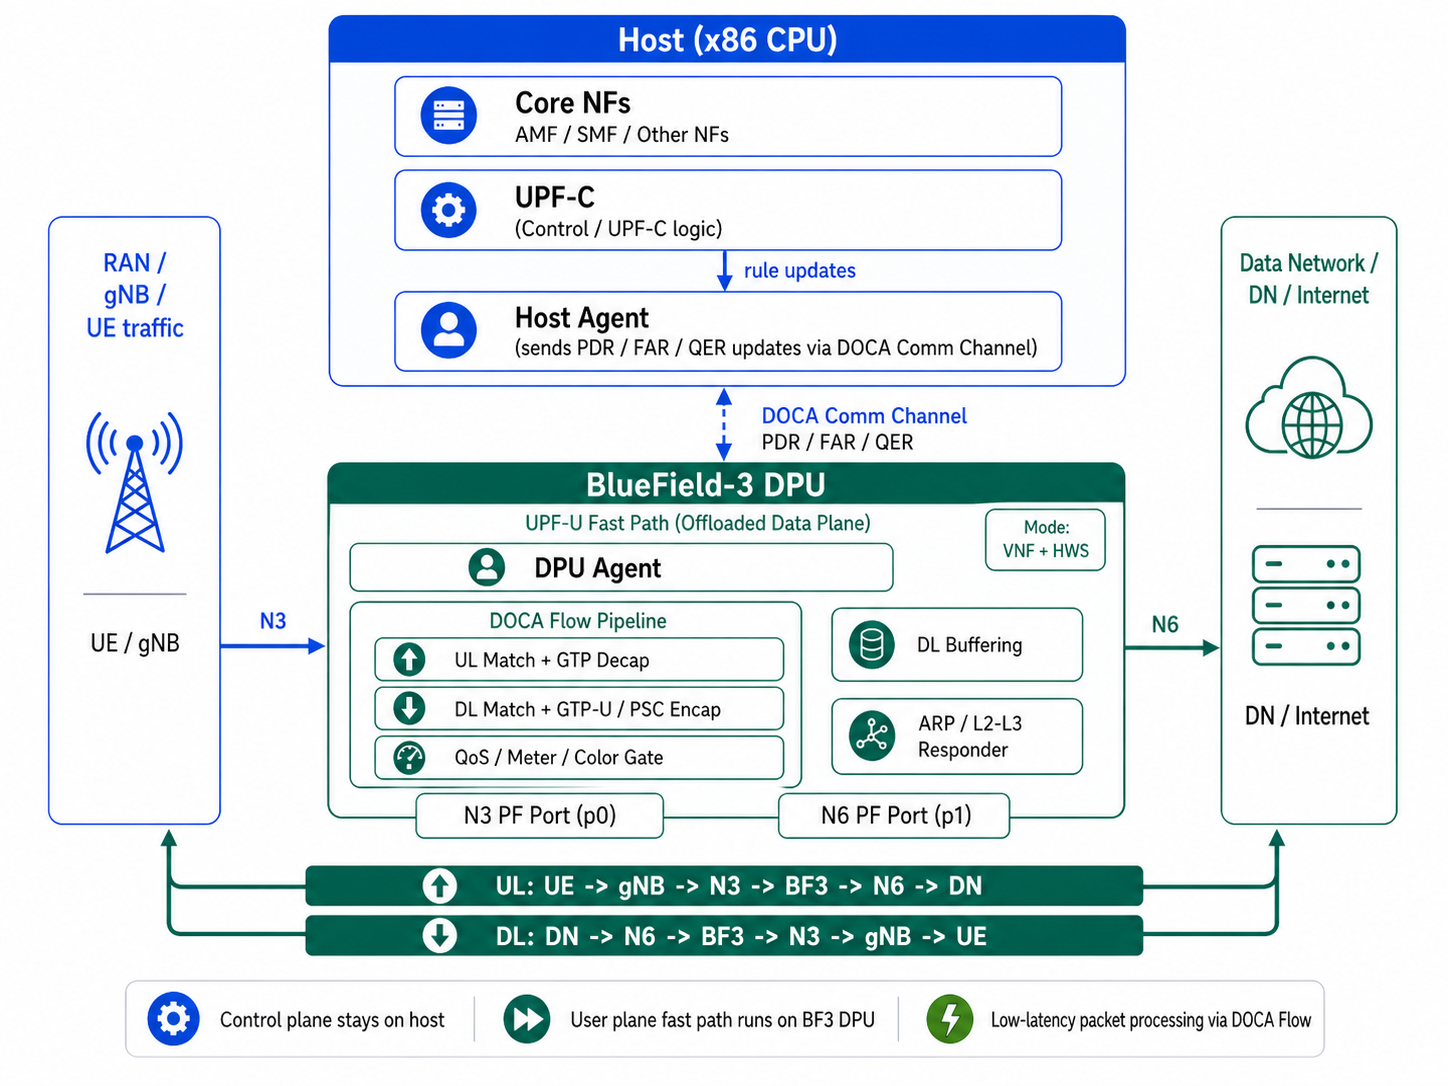
\includegraphics[width=0.98\textwidth,keepaspectratio]{images/arch.png}
  \caption{Split-agent control path: UPF-C $\to$ host\_agent $\to$ dpu\_agent.}
  \label{fig:arch}
\end{figure*}

\subsection{Cross-Domain Message: \texttt{hw\_offload\_msg\_t}}

UPF-C translates each PFCP PDR/FAR/QER event into a flat 128-byte C struct
(\texttt{hw\_offload\_msg\_t}) and enqueues it onto an ONVM inter-NF ring.
The struct carries:
\begin{itemize}
  \item \textbf{Op-code}: \texttt{CREATE}, \texttt{DELETE},
        \texttt{UPDATE\_FAR}, \texttt{UPDATE\_QER}, \texttt{UPDATE\_PDR}.
  \item \textbf{Match fields}: direction, TEID, UE IPv4, QFI, SDF 5-tuple.
  \item \textbf{FAR fields}: apply action (\texttt{FORW}/\texttt{BUFF}/
        \texttt{DROP}), outer header creation params (gNB IP, TEID, QFI).
  \item \textbf{QER fields}: MBR and GBR in kbps (uplink and downlink).
  \item \textbf{hw\_rule\_id}: A globally unique 32-bit identifier assigned
        by UPF-C via an atomic counter.  This key correlates PFCP sessions to
        DOCA Flow entries and is stamped into every packet as
        \texttt{pkt\_meta} for cross-pipe correlation.
\end{itemize}

\subsection{Host Agent}

The host\_agent is a lightweight ONVM network function whose sole
responsibility is to relay \texttt{hw\_offload\_msg\_t} structs from
the ONVM ring to the dpu\_agent over DOCA Comch (PCIe control
channel).  It performs no data-plane processing.  If the dpu\_agent
is not yet running, Comch send failures are non-fatal: rules simply
do not reach the BF3 and traffic stays on the host's existing
software path until the dpu\_agent is up and rules are
re-installed.

\subsection{DPU Agent}

The dpu\_agent is a standalone DOCA application running natively on the BF3
ARM cores.  It:
\begin{enumerate}
  \item Receives rule messages via a DOCA Comch server.
  \item Translates each message into DOCA Flow pipe entry operations
        (insert, update, delete).
  \item Manages four concurrent lcores: main (Comch + dispatch), buffer
        (DL buffering), shaper (GBR token-bucket shaping), and ARP responder.
\end{enumerate}

% ─────────────────────────────────────────────────────────────────────
\section{DOCA Flow Pipeline}
\label{sec:pipeline}

The pipeline runs in \texttt{vnf,hws} mode with two physical ports: N3
(PF0) and N6 (PF1).  There is no switch manager; each port owns its own
independent pipe domain.

\subsection{Uplink (UL) Pipeline}

GTP-U packets from the gNB arrive on the N3 wire.  The UL pipeline processes
them as follows:

\begin{enumerate}
  \item \textbf{N3\_ROOT (CONTROL, root)}: A root control pipe on N3.
        It steers packets with \texttt{UDP dst = 2152} to the
        UL\_MATCH stage.  ARP frames are steered to the ARP
        responder.  Anything else takes the default VNF miss path
        (RSS on N3) and is delivered to the host.

  \item \textbf{UL\_MATCH (BASIC, chained)}: Matches uplink packets by
        \texttt{TEID} and \texttt{UE source IP}.  On match, it stamps
        \code{pkt_meta=htonl(hw_rule_id)} and attaches a shared
        trTCM meter (RFC~2698) for QoS enforcement.  The matched entry
        forwards to the appropriate color gate.

  \item \textbf{UL\_COLOR\_GATE (BASIC)}: Interprets the meter color.  For
        non-GBR (policed) flows: GREEN and YELLOW are forwarded; RED is
        dropped.  For GBR (shaped) flows: GREEN is forwarded; YELLOW is
        diverted to the ARM shaper lcore via RSS; RED is dropped.

  \item \textbf{UL\_DECAP (BASIC)}: Strips the GTP-U outer header
        (Ethernet + IPv4 + UDP + GTP-U + PSC extension).  Prepends the N6
        Ethernet header (\code{UPF_N6_MAC} $\to$ \code{DN_GW_MAC}).
        Forwards to the N6 wire via \texttt{FWD\_PORT(N6)}.
\end{enumerate}

Packets that do not match any UL\_MATCH entry fall through the
chained pipe sequence to the default VNF miss (RSS on N3), where
the host stack handles them.

\subsection{Downlink (DL) Pipeline}

IPv4 packets from the data network arrive on the N6 wire.  The DL pipeline
encapsulates them with GTP-U and forwards them toward the gNB on N3.

\begin{enumerate}
  \item \textbf{N6\_ROOT (CONTROL, root)}: A root control pipe on N6.
        It steers IPv4 frames to the DL\_MATCH stage.  ARP frames are
        steered to the ARP responder.  Unmatched traffic takes the
        default VNF miss path (RSS on N6) and is delivered to the
        host.

  \item \textbf{DL\_MATCH (BASIC, chained)}: Matches downlink packets by
        \texttt{UE destination IP}.  On match, it stamps
        \code{pkt_meta=htonl(hw_rule_id)} and attaches the shared
        trTCM meter.  The matched entry forwards to the color gate, or to
        the ARM buffer lcore if the rule is in \texttt{BUFF} mode.

  \item \textbf{DL\_COLOR\_GATE (BASIC)}: Same color semantics as UL:
        GREEN and YELLOW forwarded (policed) or GREEN forwarded and YELLOW
        to shaper (shaped); RED dropped.

  \item \textbf{DL\_ENCAP (BASIC, EGRESS root on N3)}: Matches incoming
        packets by \texttt{pkt\_meta} and prepends the complete GTP-U outer
        header: Ethernet + IPv4 + UDP + GTP-U fixed header + optional-word
        + GTP-PSC DL extension (carrying QFI).  The encap parameters (gNB
        IP, TEID, QFI) are per-entry changeable.

        This pipe lives on the \textbf{N3 EGRESS domain} (not the DEFAULT
        domain) because hardware GTP encapsulation in the DEFAULT domain was
        found to produce malformed packets (GTP length field = 0, ephemeral
        UDP source port).  Moving it to the EGRESS root resolved this.
        A passthrough pipe (\code{N3_EGRESS_PASSTHROUGH}) is installed
        as \texttt{fwd\_miss} of DL\_ENCAP so that non-DL software-Tx
        traffic (ARP replies, buffer-drain packets) can still exit the N3
        wire unmodified.
\end{enumerate}

\subsection{Pipeline Summary}

Table~\ref{tab:pipeline} summarizes the full pipe inventory.

\begin{table*}[t]
  \centering
  \caption{DOCA Flow Pipe Inventory}
  \label{tab:pipeline}
  \begin{tabular}{@{}llll@{}}
    \toprule
    Pipe & Port & Domain & Purpose \\
    \midrule
    N3\_ROOT          & N3    & DEFAULT (root) & Steer UL GTP-U traffic; ARP frames to responder \\
    N6\_ROOT          & N6    & DEFAULT (root) & Steer DL IPv4 traffic; ARP frames to responder \\
    UL\_MATCH[0--3]   & N3    & DEFAULT        & Uplink: match on TEID + UE IP; stamp pkt\_meta; attach meter \\
    DL\_MATCH[0--3]   & N6    & DEFAULT        & Downlink: match on UE destination IP; stamp pkt\_meta; attach meter \\
    UL\_COLOR\_GATE   & N3    & DEFAULT        & trTCM color dispatch (uplink) \\
    DL\_COLOR\_GATE   & N6    & DEFAULT        & trTCM color dispatch (downlink) \\
    UL\_DECAP         & N3    & DEFAULT        & Strip GTP-U outer header; inject N6 Ethernet L2 \\
    DL\_ENCAP         & N3    & EGRESS (root)  & Match pkt\_meta; prepend GTP-U + PSC outer header; exit N3 wire \\
    N3\_EG\_PASS      & N3    & EGRESS         & DL\_ENCAP fwd\_miss target (passthrough for SW-Tx packets) \\
    TO\_DPU\_ARM\_DL  & N6    & DEFAULT        & BUFF mode: RSS DL packets to ARM buffer lcore \\
    \bottomrule
  \end{tabular}
\end{table*}

% ─────────────────────────────────────────────────────────────────────
\section{ARP Handling}

Both N3 and N6 are operated in promiscuous mode.  ARP handling is
asymmetric:

\begin{itemize}
  \item \textbf{N3 (gNB-facing)}: ARP requests from the gNB reach the BF3
        ARM via DOCA Flow RSS.  The ARP responder lcore replies normally.

  \item \textbf{N6 (DN-facing)}: The BF3 firmware routes N6 ARP frames to
        the host PCIe representor, not to the BF3 ARM.  DN-side ARP
        probes therefore never reach the responder lcore.
\end{itemize}

To work around the N6 asymmetry, the responder lcore proactively maintains the
DN neighbor's ARP cache:
\begin{itemize}
  \item On startup: sends a gratuitous ARP (GARP) broadcast and a proactive
        unicast ARP reply to the DN gateway.
  \item Periodically (every 3~s): re-sends the unicast ARP reply to keep
        the DN gateway's neighbor entry in the \texttt{REACHABLE} state.
\end{itemize}

The DN gateway therefore keeps a valid MAC entry for the UPF N6
address even though it never receives a proper ARP reply to its
probes.

% ─────────────────────────────────────────────────────────────────────
\section{DL Packet Buffering (BUFF$\to$FORW)}
\label{sec:buffering}

\textbf{Note:} The buffering path is fully implemented but \emph{not yet
validated end-to-end on BF3 hardware.}

\subsection{Motivation}

When the SMF moves a UE to idle, it sends a \texttt{BUFF} FAR
update.  The DPU then holds arriving DL packets until the SMF sends
\texttt{FORW} (after the gNB sends a paging response with the new
F-TEID).  Buffered packets must then be delivered using the updated
gNB IP and TEID, not the stale ones from before idle entry.

\subsection{Design Strategy}

\subsubsection{BUFF Activation}

On receiving \code{HW_OP_UPDATE_FAR(BUFF)}, the main thread swaps the
DL\_MATCH entry's forwarding target from the color gate to
\texttt{TO\_DPU\_ARM\_DL}, a BASIC pipe that RSS-distributes DL packets to
N6 Rx queues 0--3.  The buffer lcore polls these queues and enqueues arriving
packets into a per-flow \texttt{rte\_ring} (capacity: 8192 packets per flow,
32768 total across all flows).  The \texttt{pkt\_meta} field (set by
DL\_MATCH) is preserved across RSS and used by the buffer lcore to identify
the flow.

\subsubsection{FORW Transition}

On receiving \code{HW_OP_UPDATE_FAR(FORW)}, the main thread executes
the following ordered protocol:

\begin{enumerate}
  \item Update the DL\_ENCAP pipe entry with the new gNB IP, TEID, and QFI
        (handover-correctness: buffered packets get the \emph{new} outer
        header, not the stale pre-handover header).
  \item Transition the buffer flow state to \texttt{DRAINING}.
  \item Wait for the buffer lcore to signal \texttt{drain\_done} (100~ms
        timeout).
  \item Swap the DL\_MATCH forwarding target back to the color gate
        (re-enabling the hardware fast path).
  \item Close the buffer flow slot.
\end{enumerate}

\subsubsection{Software GTP-U Encapsulation}

During drain, the buffer lcore has to encapsulate each buffered packet
before sending it.  Re-injecting into the hardware ingress is not an
option in VNF mode (Section~\ref{sec:bg}), so the buffer lcore calls
\code{dpu_gtp_encap_dl()} in the shared codec module
(\code{dpu_gtp_codec.c}) to prepend the full Ethernet + IPv4 + UDP +
GTP-U + PSC outer header in software, and then transmits on N3
Tx~queue~2.

The \code{RTE_MBUF_DYNFLAG_TX_METADATA} flag and \texttt{pkt\_meta}
field must be cleared before transmission.  If they are not, the
mlx5 PMD injects the rule ID as hardware pkt\_meta on N3 egress,
DL\_ENCAP re-matches the already-encapsulated packet, and the result
is a double-encapsulated frame on the wire.

% ─────────────────────────────────────────────────────────────────────
\section{GBR Traffic Shaping}
\label{sec:shaping}

\textbf{Note:} The shaping path is fully implemented but \emph{not yet
validated end-to-end on BF3 hardware.}

\subsection{Motivation}

A 3GPP GBR (Guaranteed Bit Rate) flow has both a guaranteed rate and
a higher maximum rate; traffic between the two should be admitted but
smoothed.  The trTCM meter colors this in-between traffic YELLOW; the
policed path forwards YELLOW at full rate up to MBR (admitting short
bursts above GBR), while the shaped path holds YELLOW packets in a
token bucket so the average rate above GBR stays close to MBR-GBR.

\subsection{Design Strategy}

YELLOW packets from the \code{DL_COLOR_GATE_SHAPED} or
\code{UL_COLOR_GATE_SHAPED} pipes are diverted to the ARM shaper lcore
via RSS.  The shaper lcore maintains a per-flow token bucket with excess
information rate $\text{EIR} = \text{MBR} - \text{GBR}$.  Each token-bucket
refill is computed using the hardware TSC:
\begin{equation}
  \text{add} = \text{EIR} \times \frac{\Delta t}{1\,\text{s}}
\end{equation}
where $\Delta t$ is the elapsed time since the last refill in TSC ticks.

Conforming YELLOW packets are finalized in software (same
\code{dpu_gtp_codec} helpers as the buffer path) and transmitted on the
peer egress port:

\begin{itemize}
  \item \textbf{UL YELLOW}: received on N3 shaper queues, software
        GTP-U decap, transmitted on N6.
  \item \textbf{DL YELLOW}: received on N6 shaper queues, software
        GTP-U encap, transmitted on N3.
\end{itemize}

Excess YELLOW packets that exhaust the token bucket are dropped.  Per-flow
counters (\code{passed}, \code{dropped}, \code{mal_pkt},
\code{tx_dropped}) are accessible at runtime via \code{SIGUSR1}.

If the shaper table is full at registration time, the rule
automatically downgrades to the policed color gate so it is still
served, just without per-flow shaping.

% ─────────────────────────────────────────────────────────────────────
\section{Build and Run Instructions}
\label{sec:build}

The steps below reproduce the setup end-to-end.

\subsection{Prerequisites}

\begin{itemize}
  \item A FABRIC testbed slice with three nodes (UERAN, CN, DN) as
        described in Section~\ref{sec:testbed}.  The CN node must have
        an NVIDIA BF3 ConnectX-7 DPU installed
        (\texttt{NIC\_ConnectX\_7\_100} component model in FABRIC).
  \item DOCA SDK 3.3 installed on the CN host (host-side packages:
        \texttt{doca-all}) and on the BF3 ARM (via the DPU BFB flash).
\end{itemize}

\subsection{Step 1: Provision the FABRIC Slice}

Open the FABRIC provisioning notebook
\path{artifacts/L25GC_DPU_BF3_3node_complete.ipynb}
in JupyterLab and execute all cells in order.  The notebook handles:
\begin{enumerate}
  \item Slice creation with three nodes and the correct NIC model.
  \item DOCA 3.3 installation on the CN host.
  \item BF3 BFB image flashing and DPU bootstrap (rshim).
  \item L25GC-plus 5G core and ONVM-UPF installation on the CN host.
  \item DPU-side build of \code{dpu_agent} on the BF3 ARM.
\end{enumerate}

Set \code{ACTIVE_UPF_MODE="bf3"} (the default) to activate the BF3
data path.

\subsection{Step 2: Build host\_agent and dpu\_agent (Manual)}

The host\_agent is built together with UPF-U and UPF-C as part of the
ONVM-UPF tree on the x86 host, so its binary is produced by the
existing ONVM-UPF build flow and no extra build steps are needed for it
here.  The dpu\_agent is built natively on the BF3 ARM:

\runlabel{On the BF3 ARM (SSH via rshim, default IP 192.168.100.2):}
\begin{lstlisting}[language=bash]
$ cd ~/doca-upf-dma-agent
$ rm -rf build/
$ meson setup build --buildtype=release
$ meson compile -C build
\end{lstlisting}

\subsection{Step 3: Configure dpu\_agent}

Edit the runtime config file
\path{5gc/dpu_agent/config/dpu_agent_params.json}
to match your testbed's IP addresses and MAC addresses.  The critical
fields are:

\begin{lstlisting}[language=json]
{
 "doca_program_flags": {
  "comch-pci":  "03:00.0",
  "rep-pci":    "<host-pf-rep-pci>",
  "n3-pci":     "03:00.0",
  "n6-pci":     "03:00.1",
  "upf-n3-ip":  "192.168.2.2",
  "upf-n3-mac": "cc:40:f3:8f:03:56",
  "gnb-mac":    "02:71:50:41:ec:37",
  "upf-n6-ip":  "192.168.3.2",
  "upf-n6-mac": "cc:40:f3:8f:03:57",
  "dn-gw-mac":  "0a:c1:bd:c0:9d:18"
 }
}
\end{lstlisting}

The PCI address \texttt{03:00.0} is the N3 PF on the BF3; \texttt{03:00.1}
is N6.  The \code{rep-pci} value must be the BF3-side representor of the
host PF running the host\_agent (DOCA security requirement).

\subsection{Step 4: Start the Stack}

\textbf{Startup order matters.}  The host\_agent connects to the
dpu\_agent over DOCA Comch on startup; if the dpu\_agent (or any of the
ONVM-side dependencies) is not yet running, the host\_agent will fail
to attach to the control channel and rules will not reach BF3.  The
required order is:

\begin{enumerate}
  \item Start the ONVM manager and the rest of the L25GC-plus core NFs
        on the CN x86 host (AMF, SMF, UPF-U, UPF-C, etc.).
  \item Start the dpu\_agent on the BF3 ARM.
  \item Start the host\_agent on the CN x86 host \emph{only after} the
        previous two are up.  Otherwise the host\_agent will not be
        able to connect to the Comch channel exposed by the dpu\_agent.
  \item Start UERANSIM (\code{nr-gnb} then \code{nr-ue}) on the UERAN
        node.  Once UE registration and PDU session establishment
        complete, UPF-C issues \code{HW_OP_CREATE} messages, the
        host\_agent relays them to the dpu\_agent over Comch, and DOCA
        Flow entries are installed in BF3 for both UL and DL.
\end{enumerate}

\runlabel{On the BF3 ARM (start dpu\_agent):}
\begin{lstlisting}[language=bash]
$ sudo ./build/dpu_agent -l 0-3 -- -j \
config/dpu_agent_params.json
\end{lstlisting}

\runlabel{On the CN x86 host (start host\_agent, after ONVM + core NFs + dpu\_agent are up):}
\begin{lstlisting}[language=bash]
$ ./scripts/run/run_host_agent.sh 14 \
  ./NFs/onvm-upf/5gc/host_agent/config/host_agent.yaml
\end{lstlisting}

\subsection{Step 5: Verify and Debug}

Send a SIGUSR1 to the dpu\_agent to dump pipeline state, buffer stats,
shaper stats, and ARP counters to the log:
\begin{lstlisting}[language=bash]
$ kill -SIGUSR1 $(pgrep dpu_agent)
\end{lstlisting}

For end-to-end connectivity verification, run \texttt{iperf3} or
\texttt{ping} from the UE (via UERANSIM) to the DN node.  Traffic should
flow through the BF3 hardware pipeline with no host CPU involvement on the
fast path.

\subsection{Step 6: Validate Buffering (Future)}

A standalone utility, \code{dpu_far_sender}, is provided in the
\path{5gc/dpu_far_sender/} directory.  It can manually send
\code{HW_OP_UPDATE_FAR(BUFF)} and \code{HW_OP_UPDATE_FAR(FORW)}
messages for an already-installed rule without recompiling:

\begin{lstlisting}[language=bash]
# Switch a live DL rule to BUFF mode
$ ./dpu_far_sender -f config/buff.yaml
# Later, switch the same rule back to FORW
$ ./dpu_far_sender -f config/forw.yaml
\end{lstlisting}

Combine with \code{tcpdump} on N3/N6 and \code{SIGUSR1} buffer-stats
dumps to validate the drain behavior end-to-end.

% ─────────────────────────────────────────────────────────────────────
\section{Throughput Evaluation}
\label{sec:throughput}

We measured the BF3 datapath's bidirectional throughput in two
phases.  The first phase used a DN-side ONVM \code{dn_app} as a
software reflector to bounce traffic back from the DN node.  The
second phase replaced the reflector with an independent DN-side
Pktgen so that both UL and DL exercise only the BF3 hardware path.

\subsection{Methodology}

The forward traffic topology was:

\begin{lstlisting}
UE/Pktgen -> N3 -> BF3 UPF hardware -> N6 -> DN
\end{lstlisting}

Addressing summary: UE IP \code{10.60.0.1}; UPF~N3
\code{192.168.2.2}; UPF~N6 \code{192.168.3.2}; gNB IP
\code{192.168.2.1}; DN IP \code{192.168.3.1}.

In every test UE-side Pktgen replays a GTP-U PCAP toward N3.  The BF3
does UL match + GTP-U decap and forwards the inner packet on N6.  The
return direction (N6 $\to$ N3) differs between the two phases:

\begin{itemize}
  \item \textbf{Phase 1 (DN reflector)}: the DN node runs the ONVM
        manager with the \code{dn_app} NF.  \code{dn_app} reflects
        each received packet by swapping Ethernet and IPv4 source /
        destination fields and re-transmitting on the same DN port.
        The return path goes through ONVM ring scheduling, NF
        metadata, and the \code{dn_app} reflector before re-entering
        BF3 on N6 as plain DL traffic, where DL\_MATCH + DL\_ENCAP
        re-encapsulate it back toward the gNB on N3.

  \item \textbf{Phase 2 (two-sided Pktgen)}: the DN node runs its own
        Pktgen and generates plain (decapsulated) N6 packets directly
        toward BF3.  ONVM and \code{dn_app} are out of the return
        path, so UL and DL stress the BF3 hardware independently.
\end{itemize}

The DN-side reverse PCAP in Phase~2 is a plain Ethernet/IPv4 frame
(\code{src=DN_MAC}, \code{dst=UPF_N6_MAC}, \code{src=DN_IP},
\code{dst=UE_IP}); no TEID is included because BF3 itself handles the
DL match and GTP-U + PSC encap on the way out N3.

\subsection{Packet-Size Sweep via Padded Inner Payload}

The original GTP-U PCAP used small frames ($\sim$178~B on the
N3/GTP-U side; $\sim$138~B on the DN side after UL decap), which
stress packet rate rather than bandwidth.  To probe bandwidth at
larger frame sizes, we padded the inner IPv4 payload inside the
GTP-U frame using the \code{--target-dn-frame-len} option of the
PCAP generator and tested DN-side frame lengths of 512~B, 1024~B, and
1400~B.

\subsection{Phase 1 Results: UE Pktgen + DN Reflector}

In Phase~1 only UE-side Pktgen statistics were observed (DN side is
the reflector NF, not Pktgen).  Results are summarized in
Table~\ref{tab:reflector}.

\begin{table*}[t]
  \centering
  \caption{Phase 1: UE-Side Pktgen with DN ONVM \code{dn_app} Reflector}
  \label{tab:reflector}
  \footnotesize
  \setlength{\tabcolsep}{4pt}
  \begin{tabular}{@{}p{0.18\textwidth}p{0.18\textwidth}cc p{0.30\textwidth}@{}}
    \toprule
    Configuration                        & Frame size                       & UE Tx (Mpps / Gbps) & UE Rx (Mpps / Gbps) & Notes \\
    \midrule
    Small pkt, DL meter active           & $\sim$178~B N3 / $\sim$138~B DN  & 28.11 / 45.43       & 1.01 / 1.66         & Metered DL return path very weak \\
    Same small pkt, no DL meter          & $\sim$178~B N3 / $\sim$138~B DN  & 30.44 / 49.19       & 4.06 / 6.70         & No meter in PDR; return improves but still reflector-limited \\
    Padded inner                         & 512~B                            & 21.04 / 96.96       & 4.05 / 18.77        & UE Tx near 100G; return still limited \\
    Padded inner                         & 1024~B                           & 11.39 / 99.15       & 3.91 / 34.17        & Return improves with size; still much lower \\
    Padded inner                         & 1400~B                           & 7.91 / 92.60        & 3.99 / 46.88        & Return improves further; still not line rate \\
    \bottomrule
  \end{tabular}
\end{table*}

In the first small-packet run, the DL rule in the PDR carried an
active meter/policer.  UE Tx reached $\sim$45~Gbps but UE Rx was
very low ($\sim$1.66~Gbps).  Re-running the same small-packet test
with a DL PDR that had no meter installed at all raised UE Tx
slightly to $\sim$49~Gbps and UE Rx to $\sim$6.7~Gbps; return
throughput was still well below hardware capacity.  Increasing the
inner-payload size (and so the DN-side frame size) raised UE Rx
further, and UE Tx scaled to near 100~Gbps for 512~B and 1024~B
frames.  UE Rx, however, stayed well under line rate at every size
we tried in Phase~1.  The remaining gap pointed at the DN-side
software reflector rather than the BF3 hardware pipeline.

\subsection{Phase 2 Results: Two-Sided Pktgen}

In Phase~2 each side independently runs Pktgen, so both Tx and Rx
counters are observed on both sides.  Results for 512~B and 1024~B
frames are summarized in Table~\ref{tab:twosided}.

\begin{table*}[t]
  \centering
  \caption{Phase 2: Two-Sided Pktgen (UE Pktgen + DN Pktgen)}
  \label{tab:twosided}
  \begin{tabular}{@{}llrrrrr@{}}
    \toprule
    Frame size & Side       & Rx (Mpps) & Rx (Gbps) & Tx (Mpps) & Tx (Gbps) & Errors \\
    \midrule
    512~B      & UE Pktgen  & 12.90 & 55.31  & 13.70 & 58.61  & 0/0 \\
               & DN Pktgen  & 12.57 & 58.31  & 12.69 & 58.47  & 0/0 \\
    \midrule
    1024~B     & UE Pktgen  & 11.58 & 97.13  & 11.97 & 100.39 & 0/0 \\
               & DN Pktgen  & 11.36 & 99.21  & 11.48 & 99.90  & 0/0 \\
    \bottomrule
  \end{tabular}
\end{table*}

Per-direction comparisons:
\begin{itemize}
  \item \textbf{512~B}: UE Tx $\sim$58.61~Gbps $\to$ DN Rx
        $\sim$58.31~Gbps; DN Tx $\sim$58.47~Gbps $\to$ UE Rx
        $\sim$55.31~Gbps.
  \item \textbf{1024~B}: UE Tx $\sim$100.39~Gbps $\to$ DN Rx
        $\sim$99.21~Gbps; DN Tx $\sim$99.90~Gbps $\to$ UE Rx
        $\sim$97.13~Gbps.
\end{itemize}

Both UL and DL hardware paths are active and forwarding at high rate.
At 512~B the experiment is packet-rate limited ($\sim$12--13~Mpps);
at 1024~B both directions reach near line rate on the 100~Gbps
full-duplex link with zero reported Tx/Rx errors.

\subsection{Findings}

\subsubsection{The BF3 hardware path is not the bottleneck}
With ONVM \code{dn_app} out of the loop, the BF3-offloaded UPF reaches
97--100~Gbps in both UL and DL for 1024~B frames.  GTP-U decap on UL
and GTP-U encap on DL both run at near line rate.

\subsubsection{The DN-side ONVM reflector was the limiting factor}
In Phase~1, UE Tx reached near 100~Gbps for larger frames while UE
Rx stayed at 18--47~Gbps.  Replacing \code{dn_app} with a DN-side
Pktgen pushed return throughput to $\sim$97~Gbps at 1024~B.  The
earlier ceiling came from the ONVM manager, NF ring traversal, and
\code{dn_app}'s single-core processing, not from BF3 DOCA.

\subsubsection{Packet size strongly affects measured Gbps}
Small frames ($\sim$170~B) stress packet rate rather than bandwidth,
which is why the early small-packet test reported low Gbps despite
high Mpps.  At 1024~B the Mpps target for 100~Gbps drops, and the BF3
hardware path reaches near-full bandwidth.

\subsubsection{Two-sided Pktgen is a cleaner methodology than DN reflection}
Running Pktgen on both endpoints isolates the BF3 datapath: UE Pktgen
exercises only the UL hardware path, and DN Pktgen exercises only the
DL hardware path.  A software reflector mixes the two and can become
the bottleneck itself, as we saw in Phase~1.

% ─────────────────────────────────────────────────────────────────────
\section{Control-Plane Benchmarking: Rule Insertion and Deletion}
\label{sec:bench}

Beyond data-plane throughput, we also measured the
\emph{control-plane} cost: how fast the dpu\_agent can insert
and delete DOCA Flow rules.  Session-setup rate in a 5G UPF is bounded
by this number, so it is worth characterizing alongside the
data-plane numbers.

The dpu\_agent ships with built-in benchmark counters
(\code{bench-insert-enable} / \code{bench-insert-count} /
\code{bench-delete-enable} / \code{bench-delete-count} JSON
parameters) that emit one summary line per N-rule window.  When
enabled, per-rule INFO logs are suppressed so logging overhead does
not pollute the measurement.  Insertion timing covers the full DOCA
Flow entry build (match + meter attach + pkt\_meta tag + forward
target).  Deletion timing covers only the HW delete call
(\code{dpu_pipeline_delete_rule}); the post-commit 50~µs NIC drain
delay and any ARM buffer quiesce are excluded.

We ran three scale points: 200{,}000~rules, 400{,}000~rules, and
2{,}000{,}000~rules, each with a benchmark window of 10{,}000~rules.
Aggregated per-window statistics are in Table~\ref{tab:bench}.

\begin{table*}[t]
  \centering
  \caption{Rule Insertion / Deletion Throughput (Per-Window Aggregate, Window = 10{,}000 Rules)}
  \label{tab:bench}
  \begin{tabular}{@{}lrrrrrr@{}}
    \toprule
    Scale (total rules) & Op     & Windows & Min (rules/s) & Avg (rules/s) & Max (rules/s) & Avg per-rule time \\
    \midrule
    200{,}000   & INSERT & 20  & 9{,}098    & 9{,}191    & 9{,}655      & 0.109~ms \\
    200{,}000   & DELETE & 20  & 930{,}274  & 974{,}206  & 1{,}010{,}333 & 0.001~ms \\
    \midrule
    400{,}000   & INSERT & 40  & 9{,}076    & 9{,}172    & 9{,}686      & 0.109~ms \\
    400{,}000   & DELETE & 40  & 754{,}726  & 787{,}248  & 817{,}697    & 0.001~ms \\
    \midrule
    2{,}000{,}000 & INSERT & 200 & 9{,}087  & 9{,}143    & 9{,}723      & 0.109~ms \\
    2{,}000{,}000 & DELETE & 200 & 728{,}331 & 784{,}134 & 811{,}986    & 0.001~ms \\
    \bottomrule
  \end{tabular}
\end{table*}

\subsection{Findings}

\subsubsection{Insertion dominates control-plane cost}
INSERT throughput is 9{,}100--9{,}200~rules/s, or about 0.109~ms per
rule.  Per-entry HW programming time in DOCA Flow is the main cost,
since each rule does a full match + meter + pkt\_meta + forward build.

\subsubsection{Insertion rate is stable as the table grows}
The average INSERT rate at 200K, 400K, and 2M scales is 9{,}191,
9{,}172, and 9{,}143~rules/s respectively --- effectively the same.
DOCA Flow insertion cost does not visibly degrade with table size in
this range.

\subsubsection{Deletion is two orders of magnitude faster than insertion}
DELETE throughput is 780{,}000--975{,}000~rules/s, or about 0.001~ms
per rule.  The tear-down path is much cheaper than the build path, and
the bench timer excludes the post-commit NIC drain delay (which is
charged to the data-plane side).

\subsubsection{Deletion shows mild scale dependence}
DELETE rate drops from $\sim$974K~rules/s at 200K scale to
$\sim$785K~rules/s at 400K and 2M (a $\sim$20\% reduction).  The
fall-off appears between 200K and 400K and then plateaus.  We have not
investigated the exact cause.

% ─────────────────────────────────────────────────────────────────────
\section{Current Status}

Table~\ref{tab:status} summarizes the status of each component of
the offload subsystem.

\begin{table}[!h]
  \centering
  \caption{Feature Status}
  \label{tab:status}
  \begin{tabular}{@{}ll@{}}
    \toprule
    Feature                     & Status \\
    \midrule
    UL fast path (GTP-U decap)  & \textbf{Stable} \\
    DL fast path (GTP-U encap)  & \textbf{Stable} \\
    trTCM metering (RFC 2698)   & \textbf{Stable} \\
    ARP responder               & \textbf{Stable} \\
    DL packet buffering         & Implemented, untested \\
    GBR traffic shaping         & Implemented, untested \\
    \bottomrule
  \end{tabular}
\end{table}

The fast path has been run end-to-end with UERANSIM-generated GTP-U
traffic and iperf3 between a simulated UE and the DN node, confirming
correct UL decap and DL encap entirely in BF3 hardware.  Two-sided
DPDK Pktgen (Section~\ref{sec:throughput}) pushes each direction to
97--100~Gbps for 1024-byte frames with zero reported packet errors.

Buffering and shaping are code-complete but not yet validated on
hardware.  The remaining work is to exercise \texttt{BUFF$\to$FORW}
and the GBR shaper lcore under real traffic.

% ─────────────────────────────────────────────────────────────────────
\section{Future Work}

\begin{enumerate}
  \item \textbf{Validate buffering}: Use \code{dpu_far_sender} to
        trigger \texttt{BUFF$\to$FORW} on a live DL rule and verify via
        \code{tcpdump} on N3 that buffered packets are drained with correct
        GTP-U encapsulation.
  \item \textbf{Validate shaping}: Run a GBR flow with a configured
        $\text{MBR} > \text{GBR}$ and verify via \code{SIGUSR1} that
        YELLOW packets are shaped at EIR and excess is dropped.
  \item \textbf{Cleanup}: Remove dead reinject ROOT entries and
        \code{REINJECT_*} constants after buffer and shaper validation.
\end{enumerate}

% ─────────────────────────────────────────────────────────────────────
\section{Conclusion}

We designed and built a hardware-offload subsystem for ONVM-UPF, the
user-plane component of L25GC-plus, on the NVIDIA BlueField-3 DPU.
A profile of the existing software UPF showed PDR classification and
DL GTP-U encapsulation together accounting for $\sim$70\% of the
per-packet fastpath cost; both stages were pushed into the BF3
ConnectX-7 steering engine via DOCA Flow.  The split-agent model
keeps PFCP control logic on the x86 host and runs DOCA Flow
programming on the BF3 ARM, connected over DOCA Comch.  The UL/DL
fast path is stable: GTP-U decap on UL and GTP-U encap on DL both
run entirely on the BF3, and two-sided DPDK Pktgen reaches line rate
on a 100~GbE PF in both directions simultaneously for 1024-byte
frames with zero reported errors.  The return-path asymmetry seen in
early tests was traced to the DN-side ONVM \code{dn_app} reflector,
not to BF3.  Control-plane benchmarks measure 9{,}100--9{,}200 rule
inserts/s and 780{,}000--975{,}000 rule deletes/s; insert rate stays
steady from 200K up to 2M rules.  DL packet buffering and GBR
token-bucket shaping are code-complete and now need end-to-end
hardware validation, which is the next milestone.

% ─────────────────────────────────────────────────────────────────────
\begin{thebibliography}{9}

\bibitem{onvm}
  W.~Zhang \emph{et al.},
  ``OpenNetVM: A Platform for High Performance Network Service Chains,''
  in \emph{Proc. ACM HotMiddlebox}, 2016.

\bibitem{l25gc}
  V.~Jain, H.-T. Chu, S.~Qi, C.-A. Lee, H.-C. Chang, C.-Y. Hsieh,
  K.~K. Ramakrishnan, and J.-C. Chen,
  ``L25GC: A Low-Latency 5G Core Network Based on High-Performance
  NFV Platforms,''
  in \emph{Proc. ACM SIGCOMM}, 2022.
  doi:\,\href{https://doi.org/10.1145/3544216.3544267}{10.1145/3544216.3544267}.

\bibitem{l25gcplus}
  Y.-S. Liu, S.~Qi, P.-Y. Lin, H.-S. Tsai, K.~K. Ramakrishnan,
  and J.-C. Chen,
  ``L25GC+: An Improved, 3GPP-Compliant 5G Core for Low-Latency
  Control-Plane Operations,''
  in \emph{IEEE Int. Conf. Cloud Networking (CloudNet)}, 2023.
  doi:\,\href{https://doi.org/10.1109/CloudNet59005.2023.10490024}{10.1109/CloudNet59005.2023.10490024}.

\bibitem{l25gc_rethink}
  Y.-Z. Lin, C.-T. Lin, P.-Y. Lin, S.~Qi, J.-C. Chen, and
  K.~K. Ramakrishnan,
  ``Rethinking 5G Core for Performance, Fairness, and Flexibility,''
  in \emph{Proc. free5GC Workshop}, 2025.  Best Paper Award.  Source:
  \url{https://github.com/nycu-ucr/L25GC-plus}.

\bibitem{fabric}
  I.~Baldin \emph{et al.},
  ``FABRIC: A National-Scale Programmable Experimental Network Infrastructure,''
  \emph{IEEE Internet Computing}, vol.~23, no.~6, pp.~38--47, 2019.

\bibitem{doca}
  NVIDIA,
  ``DOCA SDK Documentation,'' version 3.3,
  \url{https://docs.nvidia.com/doca/}, 2024.

\bibitem{3gpp_ts29244}
  3GPP,
  ``Technical Specification 29.244: Interface between the Control Plane and
  the User Plane Nodes,'' Release 17.

\bibitem{rfc2698}
  J.~Heinanen and R.~Guerin,
  ``A Two Rate Three Color Marker,''
  IETF RFC~2698, September 1999.

\end{thebibliography}

\end{document}
